\subsection{Recap: Runtime Variability}

\begin{frame}[fragile]{\myframetitle}
	\footnotesize
	\begin{mycolumns}[animation=none]
\begin{codetight}{}
public class Config {
	~public static boolean COLORED = true;~
	@public static boolean WEIGHTED = false;@
}
\end{codetight}
\begin{codetight}{}
public class Graph {
	...
	Edge add(Node n, Node m) {
		Edge e = new Edge(n, m);
		nodes.add(n); nodes.add(m); edges.add(e);
		@if (Config.WEIGHTED) { e.weight = new Weight(); }@
		return e;
	}
	@Edge add(Node n, Node m, Weight w) {
		if (!Config.WEIGHTED) { throw new RuntimeException(); }
		Edge e = new Edge(n, m);
		nodes.add(n); nodes.add(m); edges.add(e);
		e.weight = w;
		return e;
	}@
	...
}
\end{codetight}
	\mynextcolumn
\begin{codetight}{}
public class Node {
	~Color color;~
	...
	Node(){
		~if (Config.COLORED) { color = new Color(); }~
	}
	void print() {
		~if (Config.COLORED) { Color.setDisplayColor(color); }~
		System.out.print(id);
	}
}
\end{codetight}
\begin{codetight}{}
public class Edge {
	@Weight weight;@
	...
	Edge(Node _a, Node _b) {
		a = _a; b = _b;
		@if (Config.WEIGHTED) { weight = new Weight(); }@
	}
	void print() {
		a.print(); b.print();
		@if (Config.WEIGHTED) { weight.print(); }@
	}
}
\end{codetight}
	\end{mycolumns}
\end{frame}

\begin{frame}{\myframetitle}
	\begin{mycolumns}[widths={40},T]
		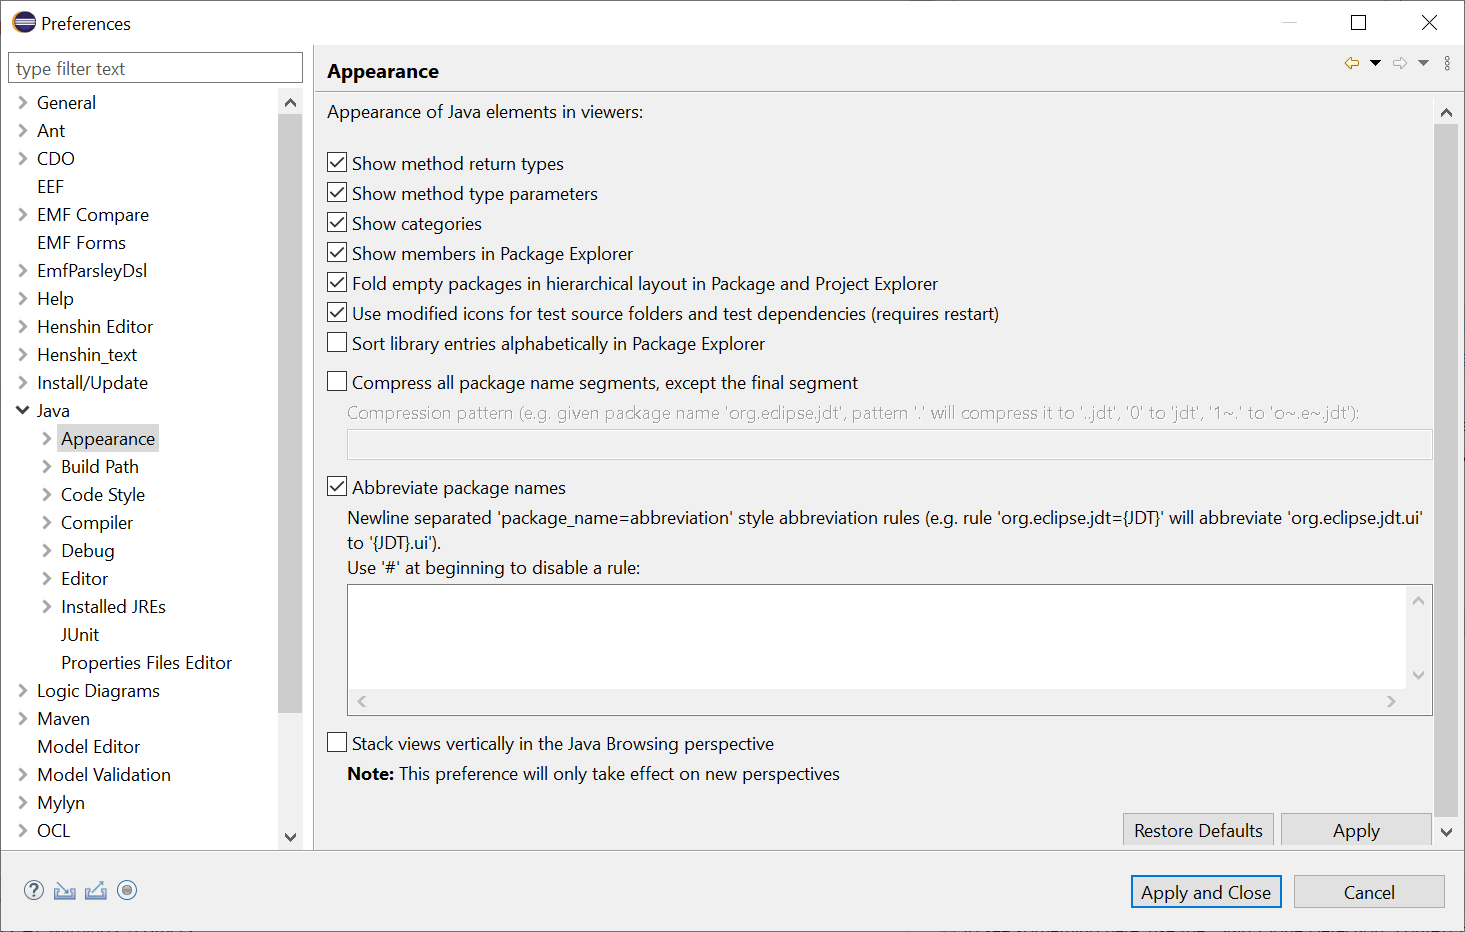
\includegraphics[width=\linewidth]{preferences-eclipse}

		\begin{definition}{How to? -- Preference Dialog}
			\begin{itemize}
				\item implement runtime variability
				\item compile the program
				\item manually adjust preferences based on configuration
				\item run the program
			\end{itemize}
		\end{definition}
	\mynextcolumn
		\leftandright{
			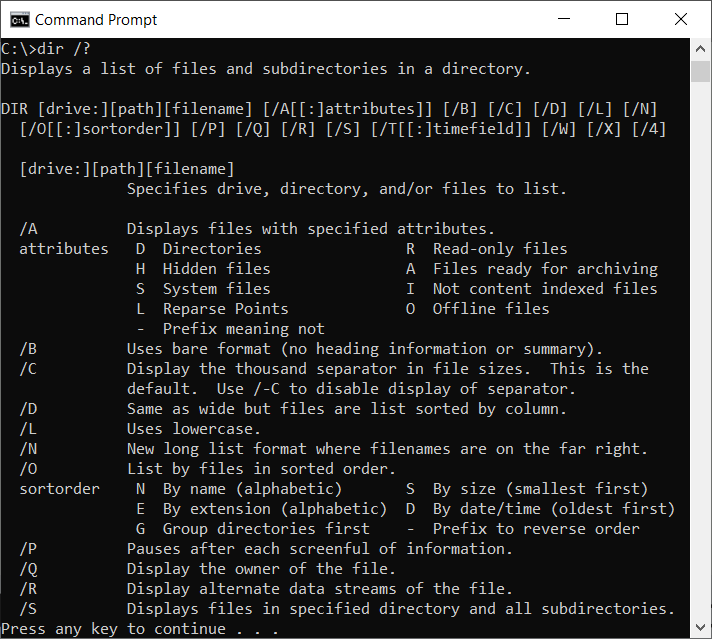
\includegraphics[width=\linewidth]{runtime-parameters-win10-cmd-dir}
		}{
			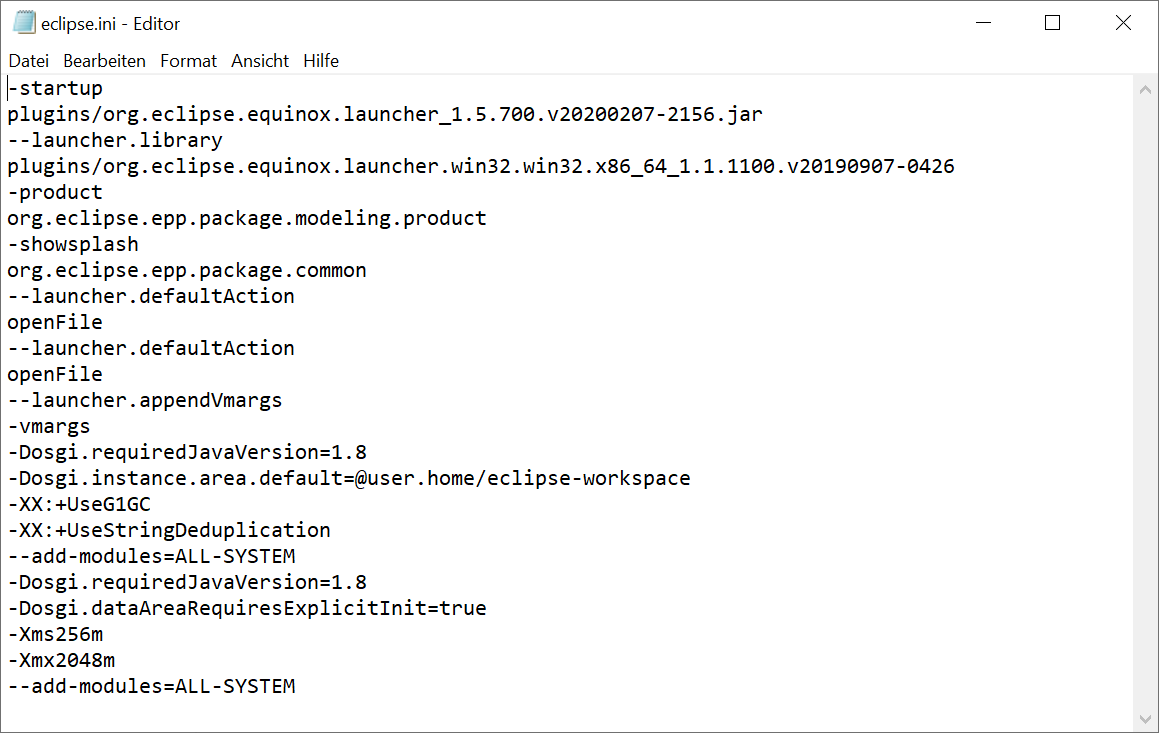
\includegraphics[width=\linewidth]{configfile-eclipse-ini}
		}

		\begin{definition}{How to? -- Command-Line Options / Configuration Files}
			\begin{itemize}
				\item implement runtime variability
				\item compile the program
				\item automatically generate command-line options / configuration files based on configuration
				\item run the program
			\end{itemize}
		\end{definition}
	\end{mycolumns}
\end{frame}

\begin{frame}[fragile]{\myframetitle}
	\begin{mycolumns}[widths={48}]
\begin{codetight}[basicstyle=\small]{}
public class Config {
	~public final static boolean COLORED = true;~
	@public final static boolean WEIGHTED = false;@
}
\end{codetight}
		\begin{definition}{How to? -- Immutable Global Variables}
			\begin{itemize}
				\item implement runtime variability
				\item automatically generate class with global variables based on configuration
				\item compile and run the program
			\end{itemize}
		\end{definition}
	\mynextcolumn
		\begin{note}{What is missing?}
			\begin{itemize}
				\item automated generation:\\\hfill for preference dialogs
				\item no compile-time variability / same large binary:\\\hfill for all except immutable global variables
				\item very limited compile-time variability:\\\hfill for immutable global variables
			\end{itemize}
		\end{note}
		\mynote{Other Problems}{
			{\bf Conditional Statements:}
			\begin{itemize}
				\item Code scattering, tangling, and replication.
			\end{itemize}	
			{\bf Design Patterns for Variability:}
			\begin{itemize}
				\item Trade-offs and potential negative side effects.
				\item Constraints that may restrict their usage.
			\end{itemize}
		}	
	\end{mycolumns}
\end{frame}

\subsection{Recap: Clone-and-Own}

\begin{frame}{\myframetitle}
	\begin{mycolumns}[columns=2,widths={50,50},animation=none]
		\mydefinition{Clone-and-Own}{
			\begin{itemize}
				\item New variants of a software system are created by copying and adapting an existing variant.
				\item Afterwards, cloned variants evolve independently of each other.
			\end{itemize}	
		}	
		\vspace{3mm}		
		\myexample{Cloning Whole Products (Clone-and-Own)}{~\hfill
\includegraphics[width=.2\linewidth]{130}\hfill
\includegraphics[width=.2\linewidth]{230}\hfill~}
	\mynextcolumn
		\pic[width=\linewidth,page=24]{lego}
	\end{mycolumns}
\end{frame}

\begin{frame}{\myframetitle}
	\begin{mycolumns}[widths={30}]
		\centering~

		
\includegraphics[scale=0.2]{alice}
		\includegraphics[scale=0.26,page=2]{graphs}

		
\includegraphics[scale=0.2]{bob}
		\includegraphics[scale=0.26,page=12]{graphs}

		
\includegraphics[scale=0.2]{eve}
		\includegraphics[scale=0.26,page=16]{graphs}
	\mynextcolumn
		\begin{definition}{How to?}
			\begin{itemize}
				\item implement separate project for each product\\(i.e., branch with version control)
				\item download project / checkout branch based on configuration
				\item run build script, if existent
				\item compile and run the program
			\end{itemize}
		\end{definition}
		\begin{note}{What is missing?}
			\begin{itemize}
				\item compile-time variability only for implemented products
				\item no automated generation:\\\hfill for clone-and-own (with version control systems)
				\item automated generation based on build script and extra files:\\\hfill for clone-and-own with build systems
				\item no free feature selection (i.e., configuration)
			\end{itemize}
		\end{note}
	\end{mycolumns}
\end{frame}

\subsection{Recap: Conditional Compilation}

\subsubsection{Preprocessors}

\begin{frame}{\myframetitle}
	\setlength\leftmargini{4mm}%
	\begin{mycolumns}[T,columns=3,animation=none]
		\begin{definition}{CPP Directives\mysource{\href{https://en.cppreference.com/w/cpp/preprocessor}{cppreference.com}}}
			file inclusion
			\begin{itemize}
				\item \texttt{\#include}
			\end{itemize}
			\only<2->{text replacement
			\begin{itemize}
				\item \texttt{\#define}
				\item \texttt{\#undef}
			\end{itemize}}
			\only<3->{conditional compilation
			\begin{itemize}
				\item \texttt{\#if}, \texttt{\#endif}
				\only<6->{\item \texttt{\#else}, \texttt{\#elif}
				\item<7-> \texttt{\#ifdef}, \texttt{\#ifndef}
				\item<8-> new: \texttt{\#elifdef}, \texttt{\#elifndef}}
			\end{itemize}}
		\end{definition}
	\mynextcolumn
		\myexampletight{Example Input}{\pic[scale=.3]{preprocessor-c}}
	\mynextcolumn
		\uncover<4->{\myexampletight{Example Output (Simplified)}{\pic[scale=.15]{preprocessor-c-output}}}
		\uncover<5->{\begin{note}{Why simplified?}
			\begin{itemize}
				\item preprocessed file can get very long due to to included header files
				\item preprocessors typically do not remove line breaks to not influence line numbers reported by compilers
			\end{itemize}
		\end{note}}
	\end{mycolumns}
\end{frame}

\begin{frame}{\myframetitle}
	\begin{mycolumns}[animation=none]
		\mynote{Advantages}{
			\begin{itemize}
				\item Well-known and mature tools, readily available
				\item Easy to use\\
				$\Rightarrow$ just annotate and remove
				\item Supports \emph{compile-time variability}
				\item Flexible, arbitrary levels of \emph{granularity}
				\item Can handle code and non-code artifacts (\emph{uniformity})
				\item Little \emph{preplanning} required\\
				$\Rightarrow$ variability can be added to an existing project
			\end{itemize}
		}
	\mynextcolumn
		\pause
		\mynote{Challenges}{
			\begin{itemize}
				\item \emph{Scattering} and \emph{tangling}\\
				$\Rightarrow$ separation of concerns?
				\item Mixes multiple languages in the same development artifact
				\item May \emph{obfuscate} source code and severely impact its readability
				\item Hard to analyze and process for existing IDEs
				\item Often used in an ad-hoc or \emph{undisciplined} fashion
				\item Prone to subtle syntax, type, or runtime errors which are hard to detect
			\end{itemize}
		}
	\end{mycolumns}
\end{frame}

\subsection{Recap: Modular Features}

\subsubsection{Components}

\begin{frame}{\myframetitle}
	\begin{mycolumns}[widths={40,60}]
		\mydefinition{General Idea}{					
			\begin{itemize}
				\item Every feature is implemented by a dedicated component.
				\item Feature selection determines which components shall be integrated to form an application.				
			\end{itemize}
		}
		\myexample{Vision}{
			\pic[width=.38\linewidth,height=1.75cm]{lego_components} 
				\vspace*{\fill}
					$\Longrightarrow$ 
				\vspace*{\fill}	
			\pic[width=.47\linewidth,height=1.75cm]{lego_product}
		}
	\mynextcolumn
		\myexample{Reality}{
			\pic[width=.27\linewidth,height=1.75cm]{lego_components} 
				\vspace*{\fill}
					$+$ 
				\vspace*{\fill}	
			\pic[width=.27\linewidth,height=1.75cm]{lego_glue}
				\vspace*{\fill}
					$=$ 
				\vspace*{\fill}	
			\pic[width=.35\linewidth,height=1.75cm]{lego_product}
		}			
		\mynote{Glue Code and Customization}{
			\begin{itemize}
				\item Developers must connect components through glue code (exception: If components are only exchanged against alternative components)
				\item Components may contain run-time variability (e.g., color manager in our example may be parameterized by color model (RGB, CMYK, ...))
			\end{itemize}
		}
	\end{mycolumns}	
\end{frame}

\subsubsection{Services}

\begin{frame}{\myframetitle}
	\begin{mycolumns}[widths={40,60},animation=none]
		\myexample{Recap: Component-Based Implementation}{
			\pic[width=.24\linewidth,height=1.0cm]{lego_components} 
				\vspace*{\fill}
					$+$ 
				\vspace*{\fill}	
			\pic[width=.24\linewidth,height=1.0cm]{lego_glue}
				\vspace*{\fill}
					$=$ 
				\vspace*{\fill}	
			\pic[width=.3\linewidth,height=1.0cm]{lego_product}
		}		
		\myexample{Plenty of Glue Code}{
			\centering
			\pic[width=.65\linewidth,height=2.5cm]{lego_glue}				
		}				
	\mynextcolumn
		\pause
		\mydefinition{Same Idea}{
			\begin{itemize}
				\item Features are implemented as services.
				\item Feature selection determines the services to be composed.
			\end{itemize}
		}	
		\pause
		\mynote{However}{
			``Standardized'' service composition instead of highly individual glue code.
		}	
		\myexample{}{
			\pic[width=.27\linewidth,height=1.75cm]{lego_components} 
				\vspace*{\fill}
					$+$ 
				\vspace*{\fill}	
			\pic[width=.27\linewidth,height=1.75cm]{lego_orchestration}
				\vspace*{\fill}
					$=$ 
				\vspace*{\fill}	
			\pic[width=.35\linewidth,height=1.75cm]{lego_product}
		}	
	\end{mycolumns}	
\end{frame}

\subsubsection{Frameworks}

\begin{frame}{\myframetitle}
	\begin{mycolumns}[widths={40,60},animation=none]
		\myexample{Recap: Service-Based Implementation}{
			\pic[width=.23\linewidth,height=1.0cm]{lego_components} 
				\vspace*{\fill}
					$+$ 
				\vspace*{\fill}	
			\pic[width=.23\linewidth,height=1.0cm]{lego_orchestration}
				\vspace*{\fill}
					$=$ 
				\vspace*{\fill}	
			\pic[width=.3\linewidth,height=1.0cm]{lego_product}
		}		
		\myexample{Still needs some specification of ``composition'' (cf.\ orchestration vs.\ choreography)}{
			\centering
			\pic[width=.65\linewidth,height=2.5cm]{lego_orchestration}				
		}				
	\mynextcolumn		
		\pause
		\mydefinition{Same Idea}{
			\begin{itemize}
				\item Features are implemented by different plug-ins
				\item Feature selection determines the plug-ins to be loaded and registered 
			\end{itemize}
		}
		\pause
		\mynote{}{
				However: Neither glue code nor explicit service composition required.
		}
		\myexample{}{
			\pic[width=.31\linewidth,height=1.75cm]{lego_product_partial} 
				\vspace*{\fill}
					$+$ 
				\vspace*{\fill}	
			\pic[width=.27\linewidth,height=1.75cm]{lego_components}
				\vspace*{\fill}
					$=$ 
				\vspace*{\fill}	
			\pic[width=.31\linewidth,height=1.75cm]{lego_product}
		}	
		\pause
		\mynote{}{
				But: Full automation comes at a price (s.\ preplanning problem).
		}			
	\end{mycolumns}	
\end{frame}

\begin{frame}{\myframetitle}
	\begin{mycolumns}[widths={50,50}]
		\myexample{}{
			In our example, we can observe that:
			\begin{itemize}
				\item There are lots of empty methods in the ColorPlugin 
				\item The Framework consults all registered plug-ins before printing a node or edge
			\end{itemize}
		}		
		\mydefinition{General Challenge: Cross-cutting Concerns}{
			Implementing cross-cutting concerns as plug-ins 
			\begin{itemize}				
				\item typically leads to huge interfaces, large parts of which are irrelevant for a dedicated plug-in 
				\item causes lots of communication overhead between plug-ins and framework
			\end{itemize}
		}
	\mynextcolumn
		\myexample{}{
			If we were not familiar with our graph library, would we anticipate that:
			\begin{itemize}
				\item Colors and weights should be part of the Plugin interface?
				\item Every plug-in needs to be notified that the framework is about to print a node or edge? 
			\end{itemize}
		}
		\mydefinition{Generally known as Preplanning Problem}{
			\begin{itemize}
				\item Hard to identify and foresee the relevant hot spots and nature of extensions
				\item Developing a framework needs lots of expertise and excellent domain knowledge 
			\end{itemize}
		}	
	\end{mycolumns}
\end{frame}


\subsection{Recap: Languages for Features}

\subsubsection{Feature-Oriented Programming}

\begin{frame}{\myframetitle}
	\begin{mycolumns}[widths={65,35},animation=none]
		\mydefinition{Feature Modules}{
			\begin{itemize}
				\item Each collaboration maps to a feature and is called a feature module (or layer).
				\item Feature modules may refine a base implementation by adding new elements or by modifying and extending existing ones.
			\end{itemize}
		}
	\mynextcolumn
		\mydefinition{Feature Module Composition}{
			Selected feature modules may be superimposed by lining-up classes according to the roles they play.
		}
	\end{mycolumns}
	\myexampletight{}{
		\centering
		\pic[width=0.95\linewidth]{feature-modules}
	}
\end{frame}

\begin{frame}{\myframetitle}
	\begin{mycolumns}[widths={50,50},animation=none]
		\mynote{Advantages}{
			\begin{itemize}
				\item Easy to use language-based mechanism, requires only minimal language extensions.
				\item Conceptually uniformly applicable to code and noncode artifacts.
				\item Separation of (possibly crosscutting) feature code into distinct feature modules.
				\item Little preplanning required due to mixin-based extension mechanism.
				\item Direct feature traceability from a feature to its implementation in a feature module.
			\end{itemize}
		}
	\mynextcolumn
		\mynote{Disadvantages}{
			\begin{itemize}
				\item Requires adoption of a language extension and composition tools.
				\item Tools need to be constructed for every language (although with the help of a framework).
				\item Only academic tools so far, little experience in practice.
				\item Granularity restricted to method-level (or other named structural entities).
			\end{itemize}
		}
	\end{mycolumns}
\end{frame}



\subsubsection{Aspect-Oriented Programming}

\begin{frame}[fragile]{\myframetitle}
	\begin{mycolumns}[widths={45,55},animation=none]
		\mydefinition{Basic Idea}{
			\begin{itemize}
				\item Implement one aspect per feature.
				\item Feature selection determines the aspects which are included in the weaving process.
			\end{itemize}
		}
		\mynote{}{
			\begin{itemize}
				\item Aspects encapsulate changes to be made to existing classes. 
				\item However, aspects do not encapsulate new classes introduced by a feature (only nested classes within an aspect)\\
					\emph{$\Rightarrow$ Gives rise to a combination of FOP and AOP.}
			\end{itemize}
		}
	\mynextcolumn
\begin{codetight}{A Color Feature for Graphs}
aspect ColorFeature {
	Color Node.color = new Color();
	
	before(Node n): execution(void print()) && this(n) {
		Color.setDisplayColor(n.color);
	}
	
	static class Color {
		...
	}
}
\end{codetight}	
	\end{mycolumns}
\end{frame}

\begin{frame}{\myframetitle}
	\begin{mycolumns}[widths={50,50},animation=none]
		\mynote{Advantages}{
			\begin{itemize}
				\item Separation of (possibly crosscutting) feature code into distinct aspects.
				\item Direct feature traceability from feature to its implementation in an aspect.
				\item Little or no preplanning effort required.
				\item Fine-grained variability driven by the join-point model of the aspect-oriented language.
			\end{itemize}
		}
	\mynextcolumn
		\pause
		\mynote{Disadvantages}{
			\begin{itemize}
				\item Requires adoption of a rather complex extension mechanism (new language and paradigm).
				\item No unifying theory like no language-independent framework.
				\item Program evolution and maintenance affected by fragile-pointcut problem.
			\end{itemize}
		}
	\end{mycolumns}
\end{frame}

























\subsection{Comparison of Implementation Techniques}
\begin{frame}
	\centering
	\begin{tabular}{|p{30mm}|p{20mm}|p{20mm}|p{20mm}|p{20mm}|}
		\hline
		 & Compile-Time Variability & Features & Product \mbox{Generation} & Feature \mbox{Traceability} \\
		\hline
		Runtime \mbox{Variability} & no (very limited for immutable global variables) & yes & yes (except for preference dialogs) & no \\
		% automated generation not for preference dialogs
		% 
		\hline
		Clone-and-Own & yes (only for implemented products) & no & no (limited generation with build systems) & no \\
		\hline
		Conditional Compilation & yes & yes & yes & with tool support \\
		\hline
		Components and Services & yes & only coarse grained & no (except pure exchange) & only coarse grained \\
		\hline
		Frameworks with Plug-Ins & yes & only coarse grained & yes & only coarse grained \\
		\hline
		FOP and AOP & yes & yes & yes & yes \\
		\hline
	\end{tabular}
\end{frame}

% large table with all properties: automatic generation from feature selection, feature modularization, ...

